
\subsection{Ejercicios}
\begin{itemize}
 
\item \textbf{Ejercicio 6}  Programar un tipo de tarea TaskBatch que reciba dos parametros: total cpu y
cant bloqueos. Una tarea de este tipo debera realizar cant bloqueos llamadas bloqueantes, en
momentos elegidos pseudoaleatoriamente. En cada tal ocasion, la tarea debera permanecer
bloqueada durante exactamente un (1) ciclo de reloj. El tiempo de CPU total que utilice una
tarea TaskBatch debera ser de total cpu ciclos de reloj (incluyendo el tiempo utilizado para
lanzar las llamadas bloqueantes; no ası el tiempo en que la tarea permanezca bloqueada).

\item \textbf{Ejercicio 7} Elegir al menos dos metricas diferentes, definirlas y explicar la semantica de
su definicion. Diseñar un lote de tareas TaskBatch, todas ellas con igual uso de CPU, pero
con diversas cantidades de bloqueos. Simular este lote utilizando el algoritmo SchedRR y una
variedad apropiada de valores de quantum. Mantener fijo en un (1) ciclo de reloj el costo de
cambio de contexto y dos (2) ciclos el de migracion. Deben variar la cantidad de nucleos de
procesamiento. Para cada una de las metricas elegidas, concluir cual es el valor optimo de
quantum a los efectos de dicha metrica.

\item \textbf{Ejercicio 8} Implemente un scheduler Round-Robin que no permita la migracion de procesos
entre nucleos (SchedRR2). La asignacion de CPU se debe realizar en el momento en que se produce la carga 
de un proceso (load). El nucleo correspondiente a un nuevo proceso sera aquel
con menor cantidad de procesos activos totales (RUNNING + BLOCKED + READY). Diseñe y realice un conjunto 
de experimentos que permita evaluar comparativamente las dos implementaciones de Round-Robin.

\item \textbf{Ejercicio 9} Disenar un lote de tareas cuyo scheduling no sea factible para el algoritmo de
prioridades fijas pero sı para el algoritmo de prioridades dinamicas.

\item \textbf{Ejercicio 10} Disenar un lote de tareas, cuyo scheduling sı sea factible con el algoritmo de
prioridades fijas, donde se observe un mejor uso del CPU por parte del algoritmo de prioridades
dinamicas.
\end{itemize}
\subsection{Resultados y Conclusiones}

\subsubsection[Resolución Ejercicio 6]{Ejercicio 6}

\indent Al igual que con la tarea TaskConsola, mencionaremos nuestro implementación y acontinuación de la misma 
explicaremos ciertos puntos de la misma.\\
 \begin{verbatim}
                       void TaskBatch(int pid, vector<int> params) {
                            int total_cpu = params[0];
                            int cant_bloqueos = params[1];
                            srand(time(NULL));
                            vector<bool> uso = vector<bool>(total_cpu);
                            for(int i=0;i<(int)uso.size();i++) 
                               uso[i] = false;
	                       for(int i=0;i<cant_bloqueos;i++) {
                                   int j = rand()%(uso.size());
                                   if(!uso[j])
                                      uso[j] = true;
                                   else
                                      i--; 
                                   }
                            for(int i=0;i<(int)uso.size();i++) {
                                if( uso[i] )
                                    uso_IO(pid,1); 
                                else
                                    uso_CPU(pid, 1); 
                               }
                            }
 \end{verbatim}

 \indent Para este tipo de tarea, creamos un vector de tamaño igual a $total_cpu$ el cual tendra bool, ya sea true o false
 dependiendo del uso que se le de dentro de la tarea, ya sea uso\_IO o uso\_CPU. En caso de ser uso\_IO sera true, y sino false.\\
 Luego, utilizaremos un ciclo que ira desde 0 hasta el tamaño del vector y dependiendo el valor booleano, usará la funciones
 dadas por la catedra uso\_IO o uso\_CPU.\\
 
 \subsubsection[Resolución Ejercicio 7]{Ejercicio 7}
 Las métricas elegidas fueron:
\begin{itemize}
 \item \textbf{Turnaround}: Es el intervalo de tiempo desde que un proceso es cargado hasta que este finaliza su ejecución.
 \item \textbf{Waiting Time}: Es la suma de los intervalos de tiempo que un proceso estuvo en la cola de procesos $ready$.
\end{itemize}

\indent \indent Como las tareas TaskBatch se bloquean pseudoaleatoriamente, 
para obtener datos relevantes tomamos un promedio de las mediciones.\\
\indent A la hora de encarar la experimentación, lo que realizamos fue simular corridas con 
varios quantum para poder obtener una aproximación del efecto del $quantum$ en la ejecución del lote de tareas. 

\indent De esta aproximación, se confeccionaron gráficos de turnaround time en función del quantum, 
referente al estudio con 2 y 3 núcleos, los cuales se proveerán a continuación:\\

\indent Luego de realizar mediciones con distintos $quantum$, tomamos la decisión de trabajar con los mismos $quantum$ para cada nucleo
al trabajar con más de 1 core. (Se muestra acontinuación un gráfico para demostrar que no era una decisión acertada trabajar
con disversos $quantum$ para cada core).

\begin{center}
    	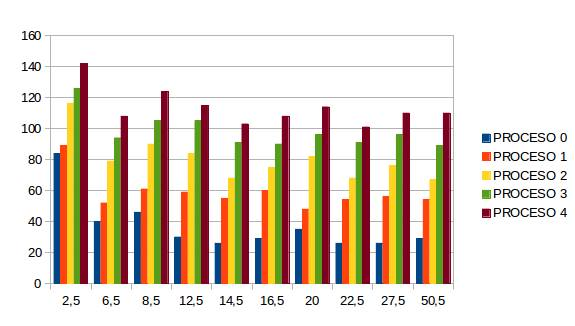
\includegraphics[width=1\textwidth]{./EJ7/turnarounddistquan.png}
	{Turnaround - 2 core - Prueba Quantum distintos por Core}\\
	{$Eje X = Quantum; $\\$ Eje Y = Tiempo$}\\
 \end{center}

\indent Al realizar, este gráfico y varias mediciones con distintos $quantum$ por core, nos dimos cuenta que no terminaban
siendo mediciones rigurosas, ya que una tarea podia estar corriendo con distintos tiempos por la migracion de procesos por core.\\
\indent Por ende, optamos por realizar mediciones con igualdad de $quantum$ por core para obtener la mejor performance posible.\\
 
 \indent Por consiguiente, al trabajar con las nuevas mediciones, conjeturamos las siguientes hipótesis:
 
 \begin{itemize}
  \item Con 2 nucleos las mediciones de tiempo tienden a estabilizarse a partir de un $quantum$ igual a 9.
  \item Con 3 nucleos las mediciones de tiempo tienden a estabilizarse a partir de un $quantum$ igual a 11.
 \end{itemize}
 \begin{center}
 \textbf{Turnaround Time} 
  \end{center}

 \begin{center}
 \textbf{2 Core}
 \end{center}
  A continuación se muestran los Diagramas de Gantt más relevantes:
  
  \begin{center}
    	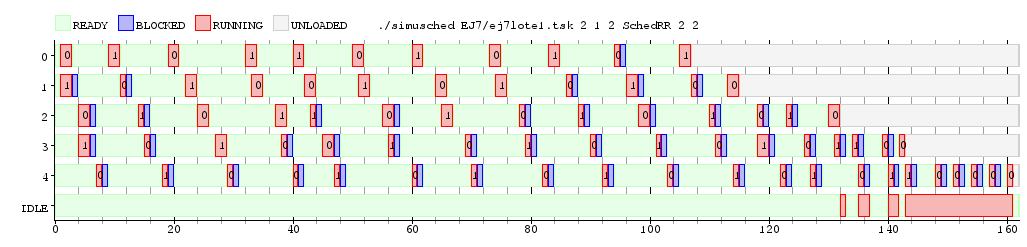
\includegraphics[width=450pt]{./EJ7/ej7tour2core1quan.png}
	{$Lote 1$ - Turnaround - 2 core - Quantum igual a 2}	
 \end{center}

   \begin{center}
    	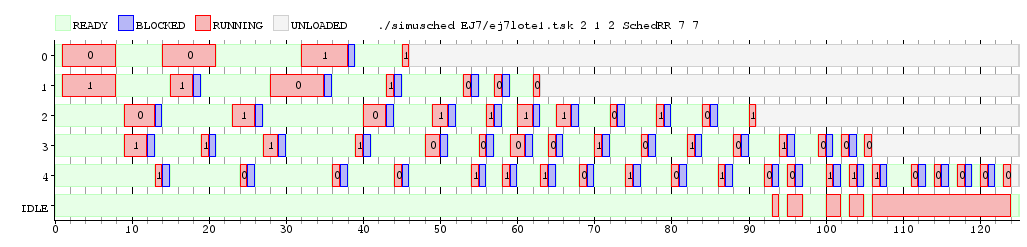
\includegraphics[width=450pt]{./EJ7/ej7tour2core3quan.png}
	{$Lote 1$ - Turnaround - 2 core - Quantum igual a 7}	
 \end{center}
 
 
 \indent La performance empieza a mejorar a medida que el $quantum$ aumenta.
 
   \begin{center}
    	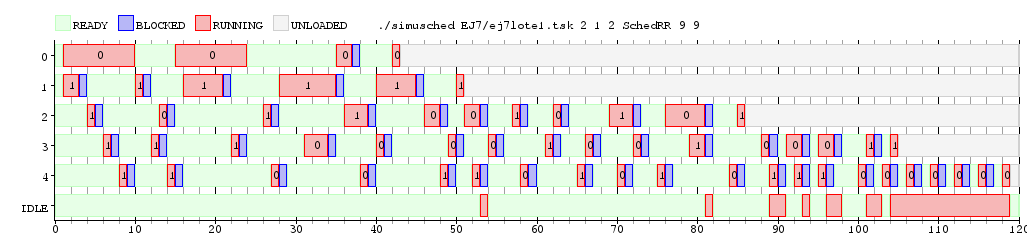
\includegraphics[width=450pt]{./EJ7/ej7tour2core4quan.png}
	{$Lote 1$ - Turnaround - 2 core - Quantum igual a 9}	
 \end{center}

  
   \indent La performance sigue mejorando,a partir de este valor, el desempeño comienza a estabilizarse, como muestran los siguiente dos gráficos. 
   Las pequeñas diferencias en los valores responden a la pseudoaleatoridad de las tareas TaskBatch.\\
  
   \begin{center}
    	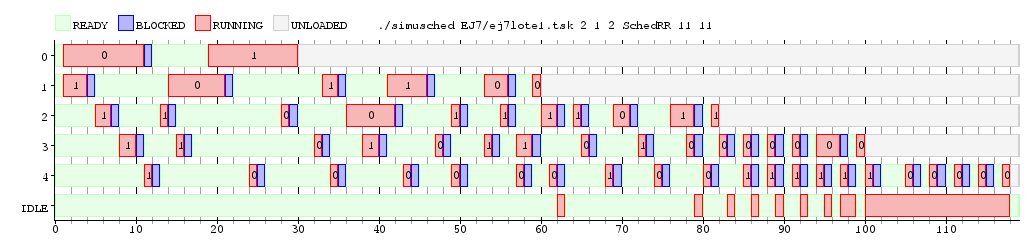
\includegraphics[width=450pt]{./EJ7/ej7tour2core5quan.png}
	{$Lote 1$ - Turnaround - 2 core - Quantum igual a 11}	
 \end{center}
 

    \begin{center}
    	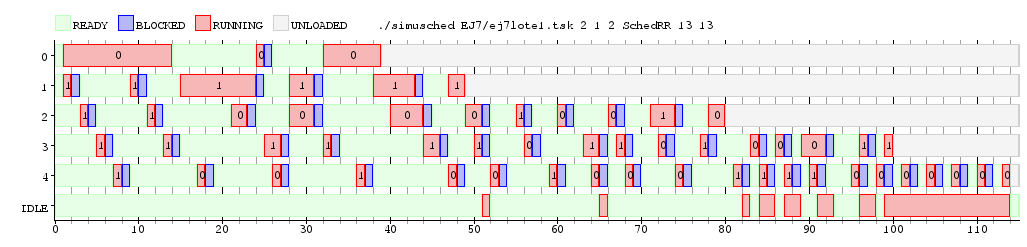
\includegraphics[width=450pt]{./EJ7/ej7tour2core8quan.png}
	{$Lote 1$ - Turnaround - 2 core - Quantum igual a 13}	
 \end{center}

 \indent Como mencionamos, las mediciones tienden a estabilizarse con un $quantum$ igual a 9, pero la mejor performance
 obtenida es con un $quantum$ igual a 13, teniendo en cuenta la pseudoaleatoridad del tipo de tarea utilizada.
 \indent Se puede observar en la primer figura que a pesar de trabajar con 2 cores, al tener un quantum bajo (igual a 2) 
 el costo es alto.\\
  
  
 \begin{center}
    	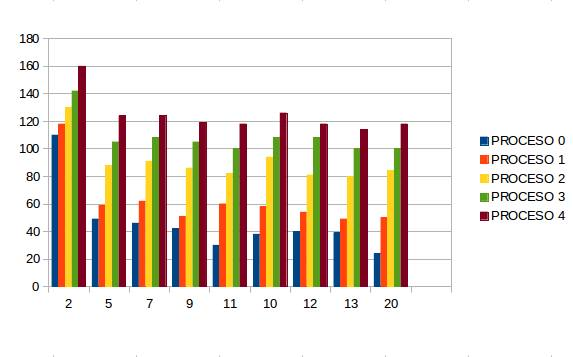
\includegraphics[width=1\textwidth]{./EJ7/tour2core.png}
	{Turnaround - 2 core}	\\
	{$Eje X = Quantum$\\$ Eje Y = Tiempo$}\\
 \end{center} 
 
 \begin{center}
  \textbf{Waiting Time}
 \end{center}

  \begin{center}
    	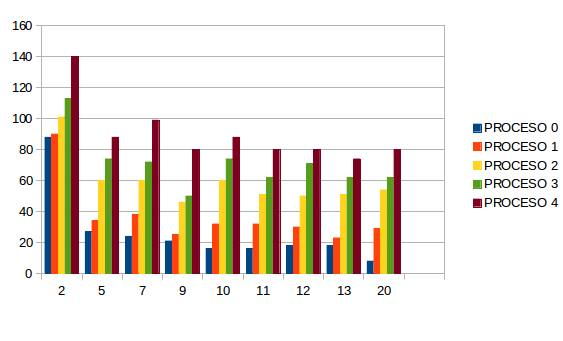
\includegraphics[width=1\textwidth]{./EJ7/waiting2core.jpg}
	{Waiting Time - 2 core}	\\
	{$Eje X = Quantum$\\$Eje Y = Tiempo$}\\
 \end{center} 
 
 \indent Con este tipo de metrica, se comienza a estabilizar a partir del $quantum$ igual a 5, obteniendo su mejor
 performance con el $quantum$ igual a 13.\\
 
   \begin{center}
   \textbf{3 Core}
   \end{center}
   \indent A continuación, al igual que con 2 cores, mostraremos los Diagramas de Gantt mas relevantes:
   
   \begin{center}
    	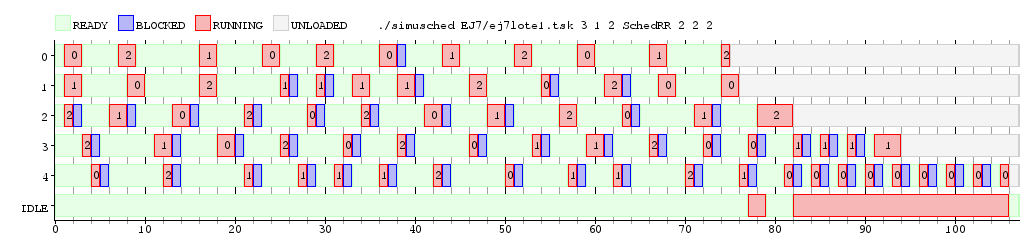
\includegraphics[width=450pt]{./EJ7/ej7tour3core1quan.png}
	{$Lote 1$ - Turnaround - 3 core - Quantum igual a 2}	
 \end{center}

 \indent Se observa que al tener otro core mas,a diferencia de con 2, a pesar de estar con un $quantum$ bajo,
 la performance mejora bastante.\\ 
 
   \begin{center}
    	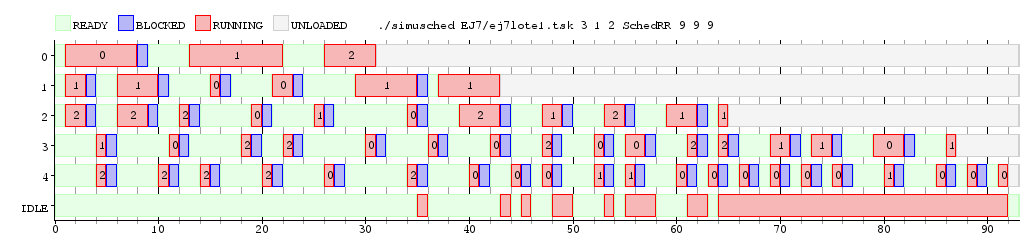
\includegraphics[width=450pt]{./EJ7/ej7tour3core4quan.png}
	{$Lote 1$ - Turnaround - 3 core - Quantum igual a 9}	
 \end{center}
 
 
 \indent La performance empieza a mejorar a medida que el $quantum$ aumenta.
 
   \begin{center}
    	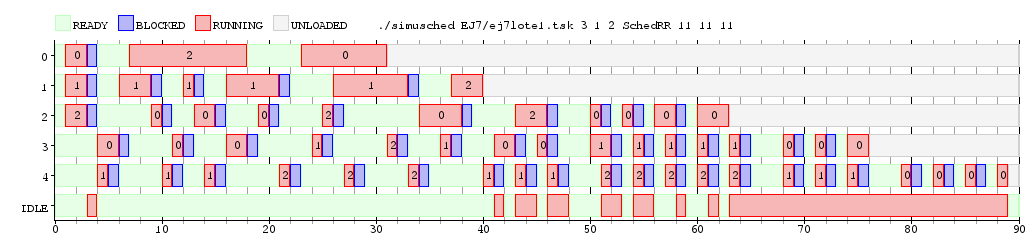
\includegraphics[width=450pt]{./EJ7/ej7tour3core5quan.png}
	{$Lote 1$ - Turnaround - 3 core - Quantum igual a 11}	
 \end{center}
  
   \begin{center}
    	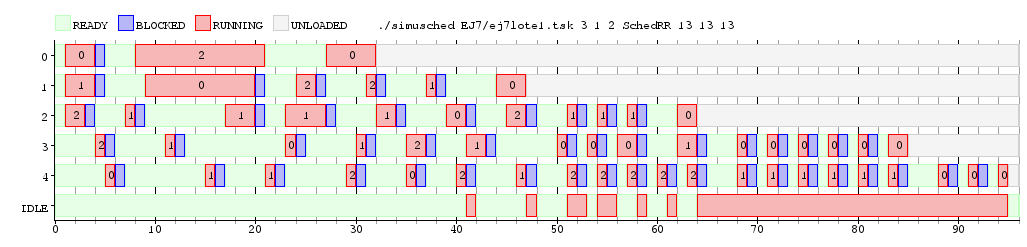
\includegraphics[width=450pt]{./EJ7/ej7tour7core6quan.png}
	{$Lote 1$ - Turnaround - 3 core - Quantum igual a 13}	
 \end{center}
 
 \begin{center}
    	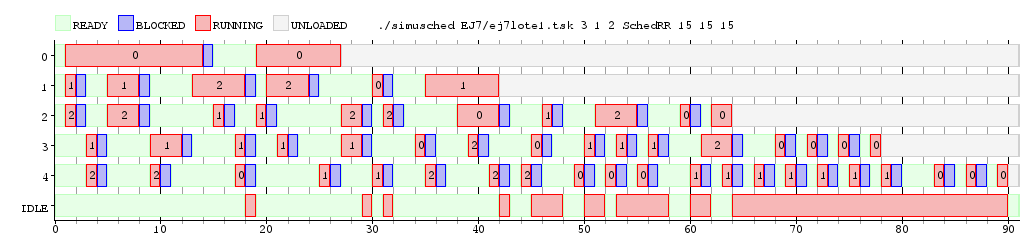
\includegraphics[width=450pt]{./EJ7/ej7tour8core6quan.png}
	{$Lote 1$ - Turnaround - 3 core - Quantum igual a 15}	
 \end{center}
 
 \indent A diferencia que en nuestra hipótesis conjeturada para con dos cores, con un $quantum$ igual a 11 se obtiene la mejor
 performance, pero teniendo en cuenta la pseudoaleatoridad del tipo de tarea con la que se trabajo, a partir del $quantum$ igual
 a 9 ya se estabiliza notoriamente.\\
   
    \begin{center}
    	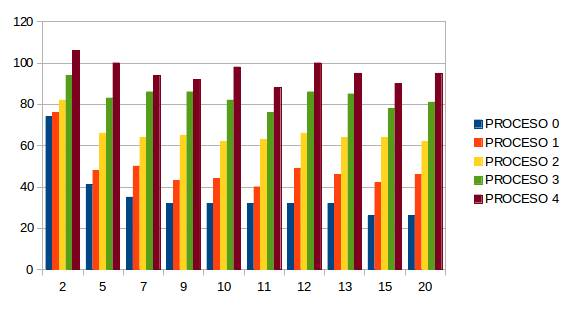
\includegraphics[width=1\textwidth]{./EJ7/tour3core.png}
	{Turnaround - 3 core}\\
	{$Eje X = Quantum $\\$ Eje Y = Tiempo$}\\
 \end{center} 
  
   \begin{center}
  \textbf{Waiting Time}
 \end{center}

  \begin{center}
    	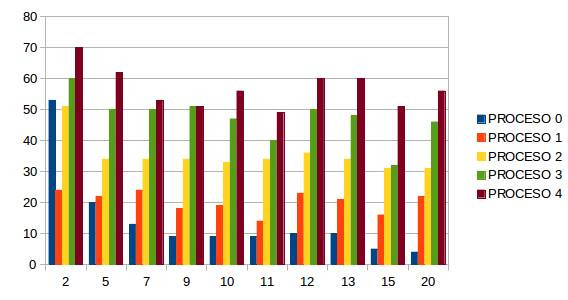
\includegraphics[width=1\textwidth]{./EJ7/waintin3core.jpg}
	{Waiting Time - 3 core}	\\
	{$Eje X = Quantum $\\$Eje Y = Tiempo$}\\
 \end{center} 
 
   \indent Con este tipo de metrica,se obteniene a diferencia de con Turnaround  su mejor
   performance con el $quantum$ igual a 15.\\
  
 \begin{center}
  \textbf{Conclusiones}
 \end{center}


\indent \indent La diferencia entre los valores de quantum entre los casos se puede atribuir a que cada vez que 
agregamos un núcleo aumentamos la posibilidad de una migración de la tareas.\\
\indent \indent En todos lo casos se observa la influencia negativa que proviene de elegir un quantum con valores pequeños.\\
\indent \indent Agregar núcleos de procesamiento mejora significativamente la performance de acuerdo a la métricas con las que
trabajamos, al permitir más procesamiento en pararelo y disminuyendo los waiting time de las tareas.\\
\indent \indent  Fijada una cantidad de núcleos, aumentar el valor del quantum también mejora la performance, 
especialmente los tiempos referidos a las tareas que menos cantidad de bloqueos tienen. 
Igualmente, a partir de cierto valor de quantum, las mejoras en la performance dejan de ser muy significativas. 
Esto se produce a que las tareas con mas cantidad de bloqueos en algun momento dejan de consumir todo
su quantum si seguimos aumentando el valor. 
 
 
 
\subsubsection[Resolución Ejercicio 8]{Ejercicio 8}

  
\subsubsection[Resolución Ejercicio 9]{Ejercicio 9}

\subsubsection[Resolución Ejercicio 10]{Ejercicio 10}
